%%%%%%%%%%%%%%%%%%%%%%%%%%%%%%%%%%%%%%%%%
% Lachaise Assignment
% LaTeX Template
% Version 1.0 (26/6/2018)
%
% This template originates from:
% http://www.LaTeXTemplates.com
%
% Authors:
% Marion Lachaise & François Févotte
% Vel (vel@LaTeXTemplates.com)
%
% License:
% CC BY-NC-SA 3.0 (http://creativecommons.org/licenses/by-nc-sa/3.0/)
% 
%%%%%%%%%%%%%%%%%%%%%%%%%%%%%%%%%%%%%%%%%

%----------------------------------------------------------------------------------------
%	PACKAGES AND OTHER DOCUMENT CONFIGURATIONS
%----------------------------------------------------------------------------------------

\documentclass{article}

%%%%%%%%%%%%%%%%%%%%%%%%%%%%%%%%%%%%%%%%%
% Lachaise Assignment
% Structure Specification File
% Version 1.0 (26/6/2018)
%
% This template originates from:
% http://www.LaTeXTemplates.com
%
% Authors:
% Marion Lachaise & François Févotte
% Vel (vel@LaTeXTemplates.com)
%
% License:
% CC BY-NC-SA 3.0 (http://creativecommons.org/licenses/by-nc-sa/3.0/)
% 
%%%%%%%%%%%%%%%%%%%%%%%%%%%%%%%%%%%%%%%%%

%----------------------------------------------------------------------------------------
%	PACKAGES AND OTHER DOCUMENT CONFIGURATIONS
%----------------------------------------------------------------------------------------

\usepackage{keystroke} % https://ctan.crest.fr/tex-archive/macros/latex/contrib/keystroke/key-test.pdf

\usepackage{amsmath,amsfonts,stmaryrd,amssymb} % Math packages

\usepackage{minted} % Code

\usepackage{enumerate} % Custom item numbers for enumerations

\usepackage{algpseudocode} % Pseudo-code package

\usepackage[ruled]{algorithm2e} % Algorithms
\SetKwInput{KwIn}{Data}
\SetKwInput{KwOut}{Output}





\usepackage[framemethod=tikz]{mdframed} % Allows defining custom boxed/framed environments

\usepackage{dirtree} % Arbre 

\usepackage{listings} % File listings, with syntax highlighting

\usepackage{xcolor}

\usepackage{graphicx}

\usepackage{hyperref}

\lstset{
	basicstyle=\ttfamily, % Typeset listings in monospace font
}

%----------------------------------------------------------------------------------------
%	DOCUMENT MARGINS
%----------------------------------------------------------------------------------------

\usepackage{geometry} % Required for adjusting page dimensions and margins

\geometry{
	paper=a4paper, % Paper size, change to letterpaper for US letter size
	top=2.5cm, % Top margin
	bottom=3cm, % Bottom margin
	left=2.5cm, % Left margin
	right=2.5cm, % Right margin
	headheight=14pt, % Header height
	footskip=1.5cm, % Space from the bottom margin to the baseline of the footer
	headsep=1.2cm, % Space from the top margin to the baseline of the header
	%showframe, % Uncomment to show how the type block is set on the page
}

%----------------------------------------------------------------------------------------
%	FONTS
%----------------------------------------------------------------------------------------

\usepackage[utf8]{inputenc} % Required for inputting international characters
\usepackage[T1]{fontenc} % Output font encoding for international characters

\usepackage{XCharter} % Use the XCharter fonts

%----------------------------------------------------------------------------------------
%	COMMAND LINE ENVIRONMENT
%----------------------------------------------------------------------------------------

% Usage:
% \begin{commandline}
%	\begin{verbatim}
%		$ ls
%		
%		Applications	Desktop	...
%	\end{verbatim}
% \end{commandline}

\mdfdefinestyle{commandline}{
	leftmargin=10pt,
	rightmargin=10pt,
	innerleftmargin=15pt,
	middlelinecolor=black!50!white,
	middlelinewidth=2pt,
	frametitlerule=false,
	backgroundcolor=black!5!white,
	frametitle={Command Line},
	frametitlefont={\normalfont\sffamily\color{white}\hspace{-1em}},
	frametitlebackgroundcolor=black!50!white,
	nobreak,
}

% Define a custom environment for command-line snapshots
\newenvironment{commandline}{
	\medskip
	\begin{mdframed}[style=commandline]
}{
	\end{mdframed}
	\medskip
}

%----------------------------------------------------------------------------------------
%	FILE CONTENTS ENVIRONMENT
%----------------------------------------------------------------------------------------

% Usage:
% \begin{file}[optional filename, defaults to "File"]
%	File contents, for example, with a listings environment
% \end{file}

\mdfdefinestyle{file}{
	innertopmargin=1.6\baselineskip,
	innerbottommargin=0.8\baselineskip,
	topline=false, bottomline=false,
	leftline=false, rightline=false,
	leftmargin=2cm,
	rightmargin=2cm,
	singleextra={%
		\draw[fill=black!10!white](P)++(0,-1.2em)rectangle(P-|O);
		\node[anchor=north west]
		at(P-|O){\ttfamily\mdfilename};
		%
		\def\l{3em}
		\draw(O-|P)++(-\l,0)--++(\l,\l)--(P)--(P-|O)--(O)--cycle;
		\draw(O-|P)++(-\l,0)--++(0,\l)--++(\l,0);
	},
	nobreak,
}

% Define a custom environment for file contents
\newenvironment{file}[1][File]{ % Set the default filename to "File"
	\medskip
	\newcommand{\mdfilename}{#1}
	\begin{mdframed}[style=file]
}{
	\end{mdframed}
	\medskip
}

%----------------------------------------------------------------------------------------
%	NUMBERED QUESTIONS ENVIRONMENT
%----------------------------------------------------------------------------------------

% Usage:
% \begin{question}[optional title]
%	Question contents
% \end{question}

\mdfdefinestyle{question}{
	innertopmargin=1.2\baselineskip,
	innerbottommargin=0.8\baselineskip,
	roundcorner=5pt,
	nobreak,
	singleextra={%
		\draw(P-|O)node[xshift=1em,anchor=west,fill=white,draw,rounded corners=5pt]{%
		Question \theQuestion\questionTitle};
	},
}

\newcounter{Question} % Stores the current question number that gets iterated with each new question

% Define a custom environment for numbered questions
\newenvironment{question}[1][\unskip]{
	\bigskip
	\stepcounter{Question}
	\newcommand{\questionTitle}{~#1}
	\begin{mdframed}[style=question]
}{
	\end{mdframed}
	\medskip
}

%----------------------------------------------------------------------------------------
%	WARNING TEXT ENVIRONMENT
%----------------------------------------------------------------------------------------

% Usage:
% \begin{warn}[optional title, defaults to "Warning:"]
%	Contents
% \end{warn}

\mdfdefinestyle{warning}{
	topline=false, bottomline=false,
	leftline=false, rightline=false,
	nobreak,
	singleextra={%
		\draw(P-|O)++(-0.5em,0)node(tmp1){};
		\draw(P-|O)++(0.5em,0)node(tmp2){};
		\fill[black,rotate around={45:(P-|O)}](tmp1)rectangle(tmp2);
		\node at(P-|O){\color{white}\scriptsize\bf !};
		\draw[very thick](P-|O)++(0,-1em)--(O);%--(O-|P);
	}
}

% Define a custom environment for warning text
\newenvironment{warn}[1][Warning:]{ % Set the default warning to "Warning:"
	\medskip
	\begin{mdframed}[style=warning]
		\noindent{\textbf{#1}}
}{
	\end{mdframed}
}

%----------------------------------------------------------------------------------------
%	INFORMATION ENVIRONMENT
%----------------------------------------------------------------------------------------

% Usage:
% \begin{info}[optional title, defaults to "Info:"]
% 	contents
% 	\end{info}

\mdfdefinestyle{info}{%
	topline=false, bottomline=false,
	leftline=false, rightline=false,
	nobreak,
	singleextra={%
		\fill[black](P-|O)circle[radius=0.4em];
		\node at(P-|O){\color{white}\scriptsize\bf i};
		\draw[very thick](P-|O)++(0,-0.8em)--(O);%--(O-|P);
	}
}

% Define a custom environment for information
\newenvironment{info}[1][Info:]{ % Set the default title to "Info:"
	\medskip
	\begin{mdframed}[style=info]
		\noindent{\textbf{#1}}
}{
	\end{mdframed}
}


%----------------------------------------------------------------------------------------
%	EQUATION
%----------------------------------------------------------------------------------------

\newcommand{\equabezier}{
	\begin{displaymath}
		P(t) = P_0(1-t)^3+3P_1t(1-t)^2+3P_2t^2(1-t)+P_3t^3	
	\end{displaymath}
} % Include the file specifying the document structure and custom commands

%----------------------------------------------------------------------------------------
%	ASSIGNMENT INFORMATION
%----------------------------------------------------------------------------------------

\title{Mathématiques pour l'Informatique : Compte Rendu} % Title of the assignment
\author{Valentin VERSTRACTE \& Evan PETIT}

\date{L3 --- Jean-Luc BARIL --- \today} % University, school and/or department name(s) and a date



%----------------------------------------------------------------------------------------

\begin{document}

\maketitle % Print the title

%----------------------------------------------------------------------------------------
%	Table des matières
%----------------------------------------------------------------------------------------
\bigskip
\bigskip
\renewcommand{\contentsname}{Table des matières}
\tableofcontents
\vspace{75pt}

%----------------------------------------------------------------------------------------
% 
%----------------------------------------------------------------------------------------

\section{Introduction} 

Ce rapport concerne le rendu du projet de Mathématiques pour l'informatique. Le projet a été intégralement réalisé en collaboration sur GitHub, en langage C++ pour l'implémentation des algorithmes, et en \LaTeX pour le compte-rendu.\\~\\
Sommaire des fonctionnalités implémentées :


\begin{description}
	\item [Transformée de Fourier discrète 1D \& 2D] Implémentation de la transformée discrète directe et inverse depuis la formule mathématique 
	\item [Transformée de Fourier rapide 1D \& 2D] Implémentation de la transformée rapide avec l'algorithme de Cooley-Tukey
	\item [Séquence de tests] Vérification des résultats obtenus 
\end{description}

\newpage

\section{Transformée de Fourier discrète}



\subsection{Transformée de Fourier 1D directe et inverse}

\subsubsection{Formule}
On rappelle la formule, où \textbf{g(x)} est le signal original, et \textbf{$\widehat{\textbf{g}}$(x)} est son calcul par la TFD. La transformée de Fourier directe permet d'obtenir $\widehat{g}$(x) depuis g(x).

\begin{equation}
		\widehat{g}(x) = \sum_{x = 0}^{N-1}g(x) exp(\frac{-2i\pi kx}{N}) \qquad pour \qquad 0 \leq k < N
\end{equation}

\noindent L'inverse permet... L'inverse. On remarque l'introduction d'une multiplication d'un facteur -1 dans l'exponentielle

\begin{equation}
	g(x) = \sum_{x = 0}^{N-1}\widehat{g}(x) exp(\frac{2i\pi kx}{N}) \qquad pour \qquad 0 \leq k < N
\end{equation}


\noindent L'algorithme équivalent peut être implémenté de façon brutale. On a besoin de deux boucles : Une pour calculer le produit à l'intérieur de la somme pour les valeurs de k allant de 0 à N-1, et une pour sommer tous les résultats obtenus pour x allant de 0 à N-1. Modulo un facteur -1 pour obtenir la transformée inverse.

Il suffit donc d'implémenter une fonction qui prend un tableau 1D et un booléen en entrée - Qui permet de choisir entre transformée directe et inverse.

\begin{algorithm}
	\caption{Transformée discrète 1D directe et inverse}\label{alg:cap}
	\KwIn{$g[N]$ : Vecteur 1D complexe\\inverse : Booléen }
	\KwOut{$G[N]$ : Vecteur 1D complexe}
	\Begin{
		\For{$k \gets 0 .. N-1$}
		{   
			$somme \gets 0$\\
			\For{$x \gets 0 .. N-1$}
			{
				$z = ( 2 * i * \Pi * k * x ) / N$\\
				\If{inverse}{$z \gets -z$}
				$somme \gets somme + g[x] * exp(z)$
			}
			$G[k] \gets somme$\\
			\If{inverse}{$G[k] \gets G[k]/N$}
		}		
	}		
\end{algorithm}

\subsubsection{Complexité}

La complexité de l'algorithme se déduit assez facilement. Soit \textbf{g} le vecteur passé en entrée, de taille \textbf{n}, et \textbf{k} un indice quelconque de g.
\begin{itemize}
	\item Pour calculer \textbf{g[k]} il faut calculer le produit de g[0] avec une exponentielle complexe, de même pour g[1], g[2], . . . , g[n-1] et faire la somme de tous ces produits. Le tableau est de taille n, on fait donc n produits ainsi qu'une addition (négligeable). On peut dire qu'on effectue \textbf{n} opérations élémentaires.
	\item Il faut répéter cette étape autant de fois qu'il y a d'indices dans le tableau. C'est à dire \textbf{n} fois.
	\item Au total on compte (à quelques constantes près) \textbf{n*n} opérations.
	La complexité finale est donc de l'ordre de O(n * n) = \textbf{O(n²)} 
\end{itemize}

\subsubsection{Diagramme}

On peut réaliser un simple diagramme pour représenter cet algorithme. Ici g[x] est le signal d'entrée (représenté par un vecteur 1D), et G[x] le vecteur en sortie. Ils sont de taille N.

\begin{figure}[!htb]
	\centering
	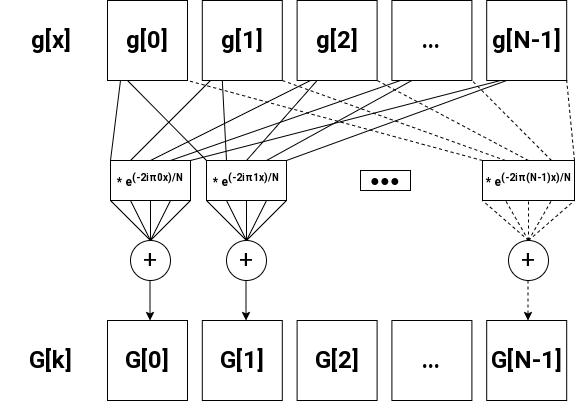
\includegraphics[height=8cm]{./assets/TFD1D.png}
	\caption{TFD 1D}
	\label{fig:TFD1D}
\end{figure}


\subsection{Transformée de Fourier 2D discrète et séparabilité}

La formule de la transformée de Fourier 2D discrète directe est la suivante :

\begin{equation}
	\widehat{g}(x,y) = \sum_{x = 0}^{N-1}\sum_{y = 0}^{M-1}g(x,y) exp(-2i\pi(\frac{jx}{N}+\frac{ky}{M})) \quad pour \quad 0 \leq j < N\quad et \quad 0 \leq k < M
\end{equation}

\noindent On admettra que la matrice d'entrée - l'image, ici - est séparable, c'est à dire que $g[x,y] = X[x]Y[y]$. 


\section{Transformée de Fourier rapide}

\section{Annexe}



\end{document}
